\section{Observation and Calculation}

	\subsection{Magnetic field calibration}

		We used an electromagnet coil of 500 turns. Then we gradually increased the current in the coil and measured the magnetic field using a Hall probe. The data is shown in Table \ref{tab:1}. The graph of B vs I is shown in Fig \ref{graph:1}.

		\begin{table}[H]
    \centering
    \begin{tabular}{|c|c|}
        \hline
        sl no. & background \\ \hline
        1      & 84         \\ \hline
        2      & 60         \\ \hline
        3      & 65         \\ \hline
        4      & 74         \\ \hline
        5      & 69         \\ \hline
        avg    & 70.4       \\ \hline
    \end{tabular}
    \label{tab:1}
    \caption{Background counts for 60s}
\end{table}
		\begin{figure}[h]
			\centering
			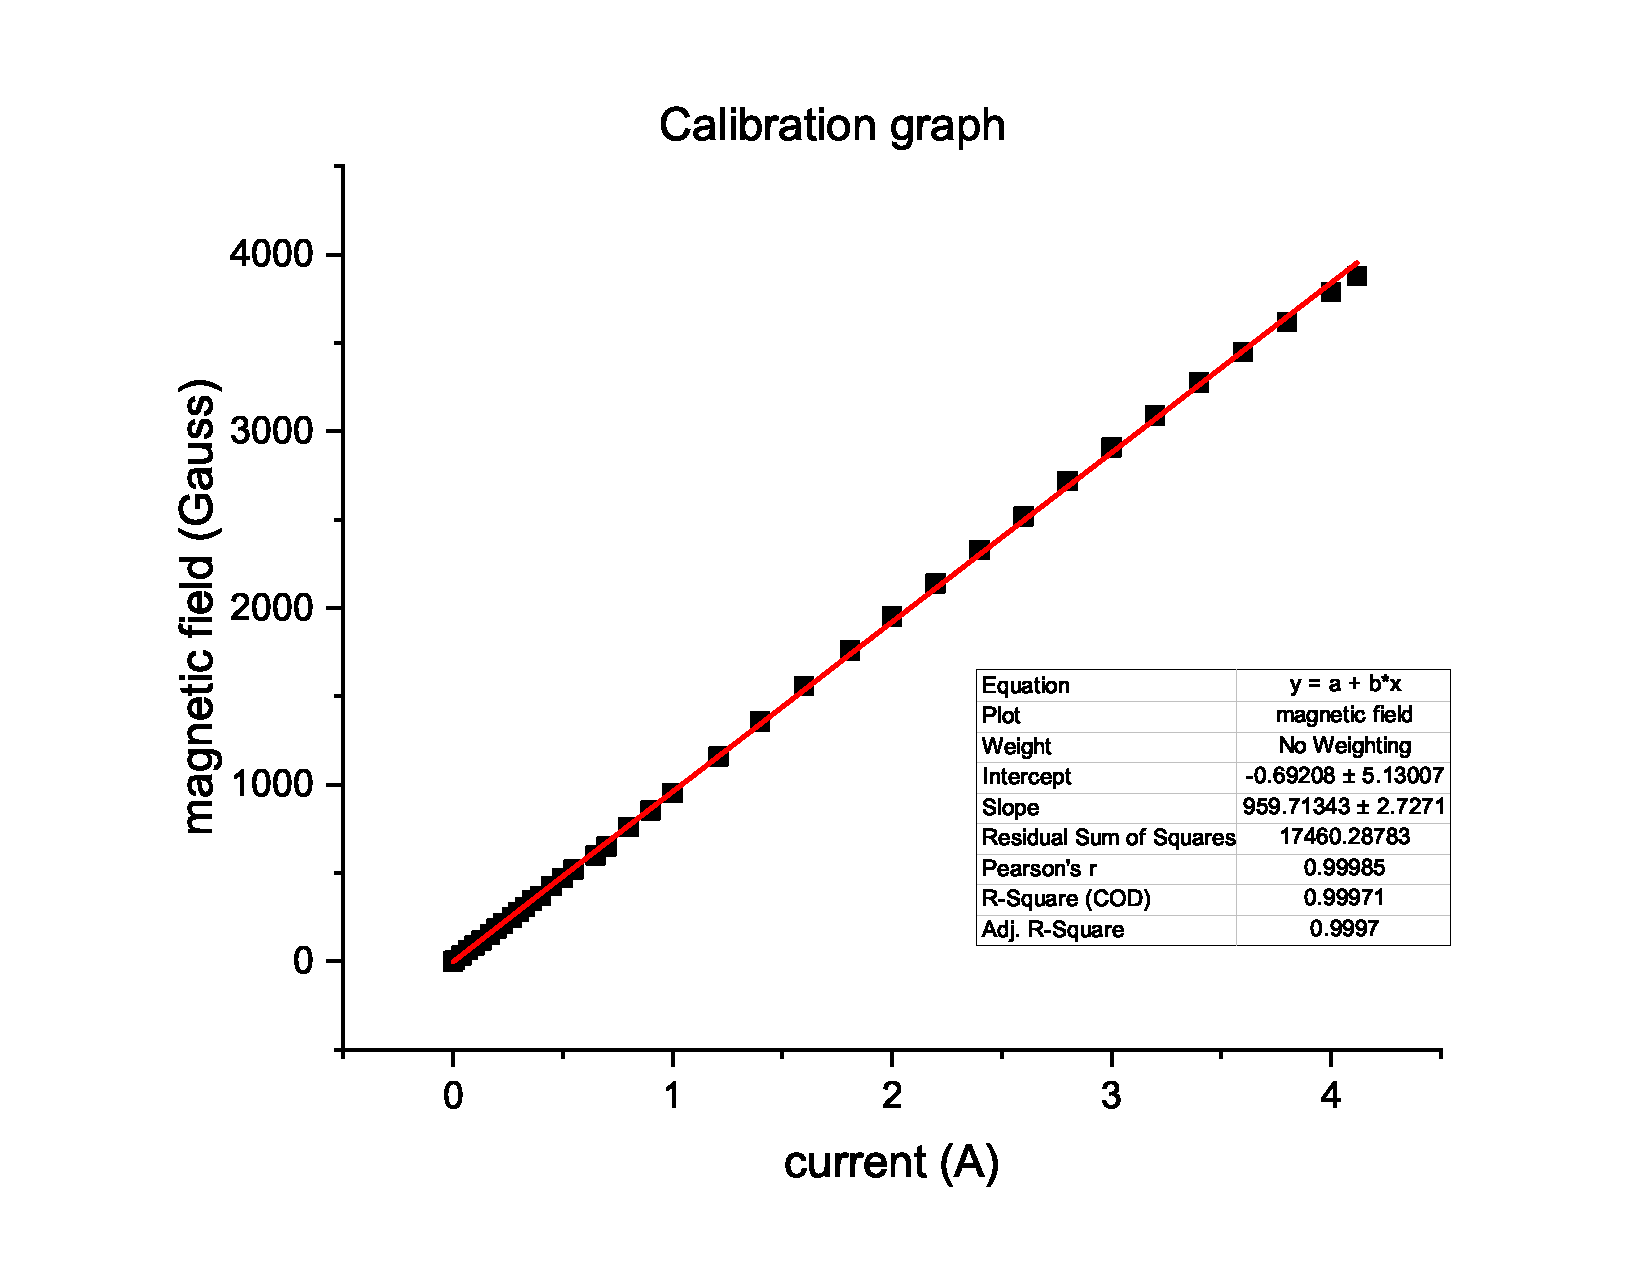
\includegraphics[width=0.8\columnwidth]{images/cal.eps}
			\caption{B vs I (coil current)}
			\label{graph:1}
		\end{figure}

	\subsection{Constant temperature}
		\subsubsection{Ge n-type}

			\begin{itemize}
				\item sample thickness = $t=0.5mm$
				\item coil current = $I=3.21A$
				\item $H=3277G$
			\end{itemize}

			We measured the Hall voltage at different probe current. The data is shown in Table \ref{tab:2}. The graph of Hall voltage vs probe current is shown in Fig \ref{graph:2}.

			from Graph \ref{graph:2}, we have $slope=\sfrac{V_y}{I_x}=-19.8$. Thus, using Equation \ref{eq:1} $ R_H=-3.02 cm^3 coulomb^{-1}$

			\begin{table}[H]
    \centering
    \begin{tabular}{|c|c|c|}
        \hline
        thickness & count & net count \\ \hline
        0         & 1216  & 204       \\ \hline
        0.6       & 853   & 783       \\ \hline
        0.12      & 706   & 636       \\ \hline
        0.18      & 504   & 434       \\ \hline
        0.24      & 420   & 350       \\ \hline
        0.3       & 311   & 241       \\ \hline
        0.36      & 222   & 152       \\ \hline
        0.42      & 199   & 129       \\ \hline
        0.48      & 168   & 98        \\ \hline
        0.54      & 145   & 75        \\ \hline
    \end{tabular}
    \label{tab:2}
    \caption{$\beta$ praticle counts for  $Tl^{204}$ in aluminium absorber}
\end{table}
			\begin{figure}[h]
				\centering
				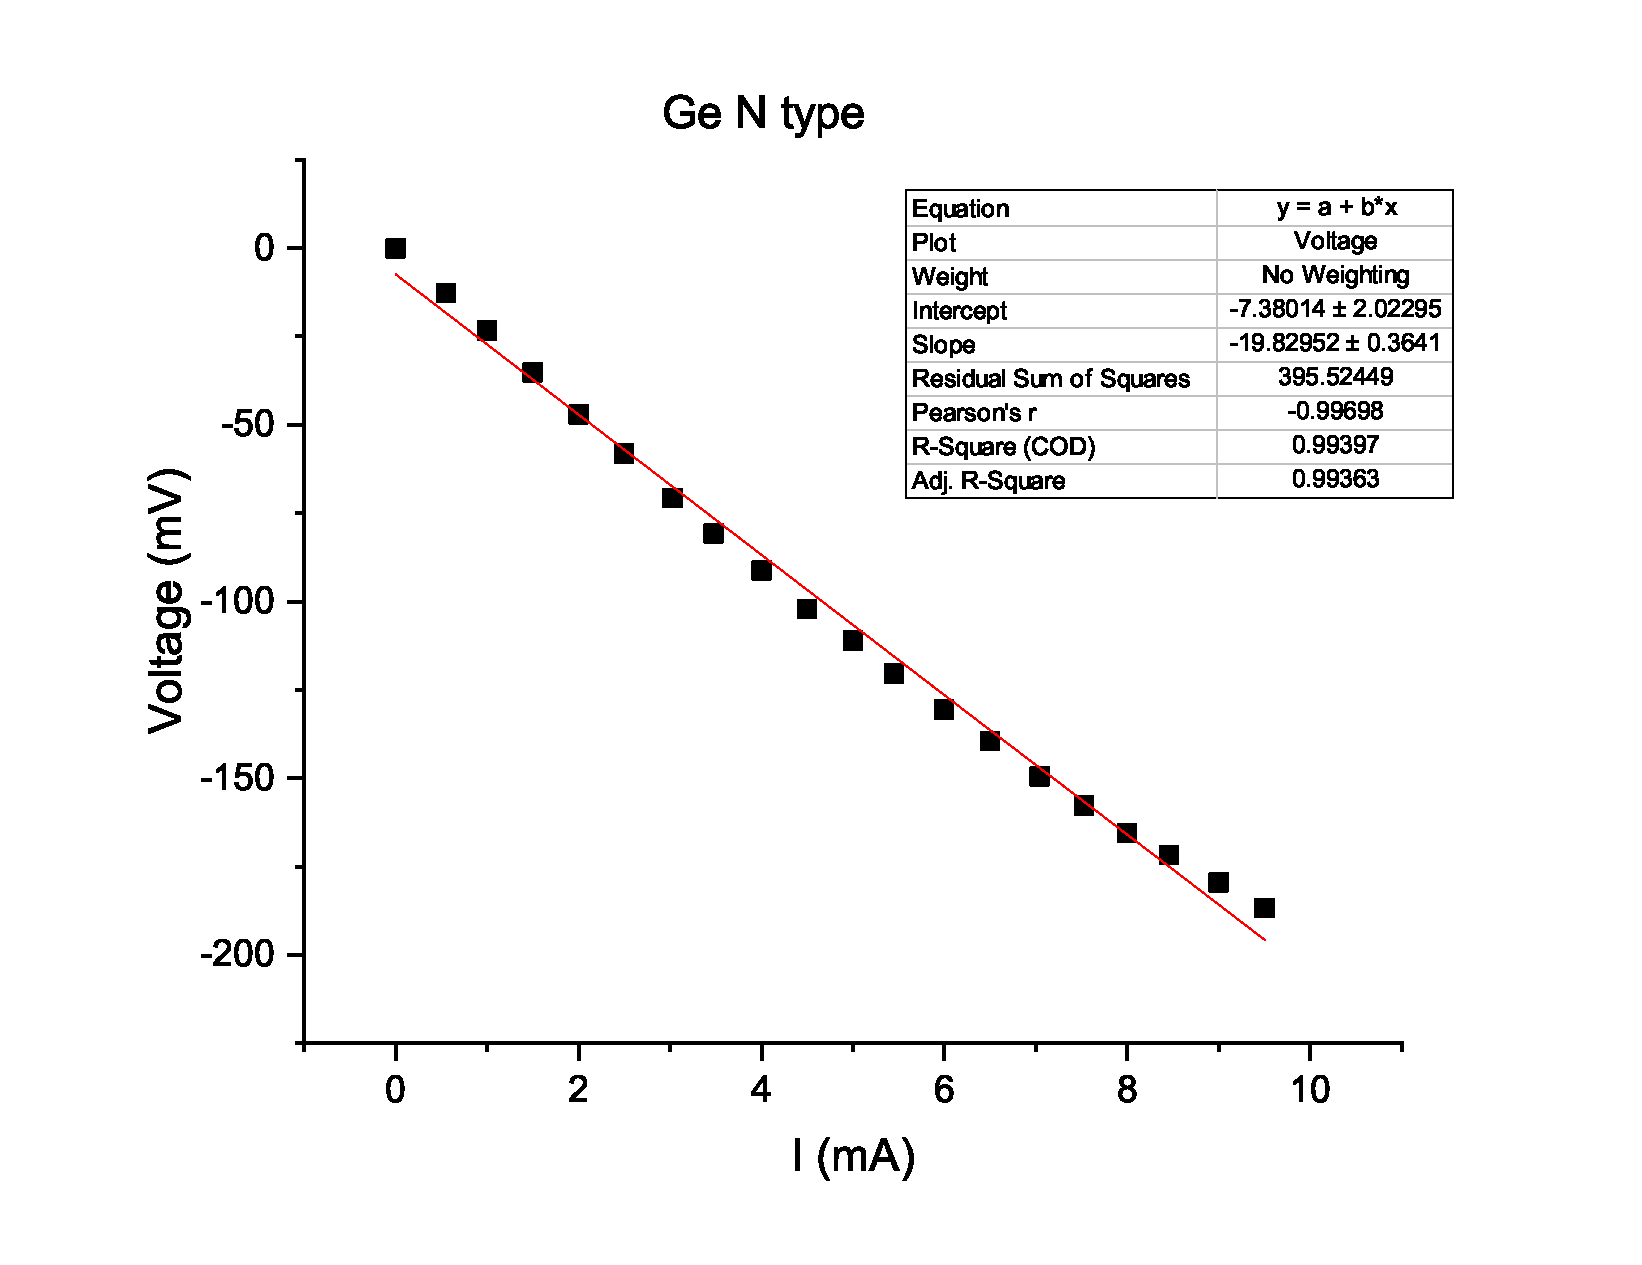
\includegraphics[width=0.9\columnwidth]{images/gen.eps}
				\caption{Hall voltage vs. probe current for Ge n-type}
				\label{graph:2}
			\end{figure}


		\subsubsection{Ge p-type}

			\begin{itemize}
				\item sample thickness = $t=0.5mm$
				\item coil current = $I=3.21A$
				\item $H=3277G$
			\end{itemize}
			
			% Please add the following required packages to your document preamble:
% \usepackage{graphicx}
\begin{table}[h]
    \centering
    \resizebox{0.75\columnwidth}{!}{%
    \begin{tabular}{|c|c|c|c|}
    \hline
    \textbf{I (mA)} & \textbf{\begin{tabular}[c]{@{}c@{}}Hall Voltage\\ (mV)\end{tabular}} & \textbf{\begin{tabular}[c]{@{}c@{}}Offset Voltage\\ (mV)\end{tabular}} & \textbf{\begin{tabular}[c]{@{}c@{}}Voltage\\ (mV)\end{tabular}} \\ \hline
    0.0 & 0 & 0 & 0 \\ \hline
    0.5 & 3.6 & -3.2 & 6.8 \\ \hline
    1.0 & 7.3 & -6.8 & 14.1 \\ \hline
    1.5 & 10.8 & -10.2 & 21.0 \\ \hline
    2.0 & 14.4 & -13.6 & 28.0 \\ \hline
    2.5 & 17.9 & -16.8 & 34.7 \\ \hline
    3.0 & 22.4 & -20.9 & 43.3 \\ \hline
    3.5 & 25.8 & -24.4 & 50.2 \\ \hline
    4.0 & 29.1 & -27.5 & 56.6 \\ \hline
    4.5 & 32.4 & -31.1 & 63.5 \\ \hline
    5.0 & 36.3 & -35.3 & 71.6 \\ \hline
    5.5 & 38.9 & -38.5 & 77.4 \\ \hline
    6.0 & 42.4 & -42.4 & 84.8 \\ \hline
    6.5 & 44.8 & -46.2 & 91.0 \\ \hline
    7.0 & 48.0 & -50.3 & 98.3 \\ \hline
    7.5 & 50.9 & -54.0 & 104.9 \\ \hline
    8.0 & 53.9 & -58.3 & 112.2 \\ \hline
    8.5 & 56.0 & -62.7 & 118.7 \\ \hline
    9.0 & 58.3 & -64.9 & 123.2 \\ \hline
    9.5 & 62.5 & -70.1 & 132.6 \\ \hline
    10.0 & 64.5 & -73.8 & 138.3 \\ \hline
    10.5 & 67.8 & -77.2 & 145.0 \\ \hline
    11.0 & 69.6 & -79.5 & 149.1 \\ \hline
    11.5 & 72.3 & -83.1 & 155.4 \\ \hline
    12.0 & 70.7 & -90.9 & 161.6 \\ \hline
    12.5 & 72.1 & -94.3 & 166.4 \\ \hline
    13.0 & 74.6 & -99.0 & 173.6 \\ \hline
    14.0 & 77.6 & -107.8 & 185.4 \\ \hline
    15.0 & 77.5 & -117.2 & 194.7 \\ \hline
    \end{tabular}%
    }
    \caption{Ge-P type hall voltage at different probe current}
    \label{tab:3}
\end{table}
			\begin{figure}[h]
				\centering
				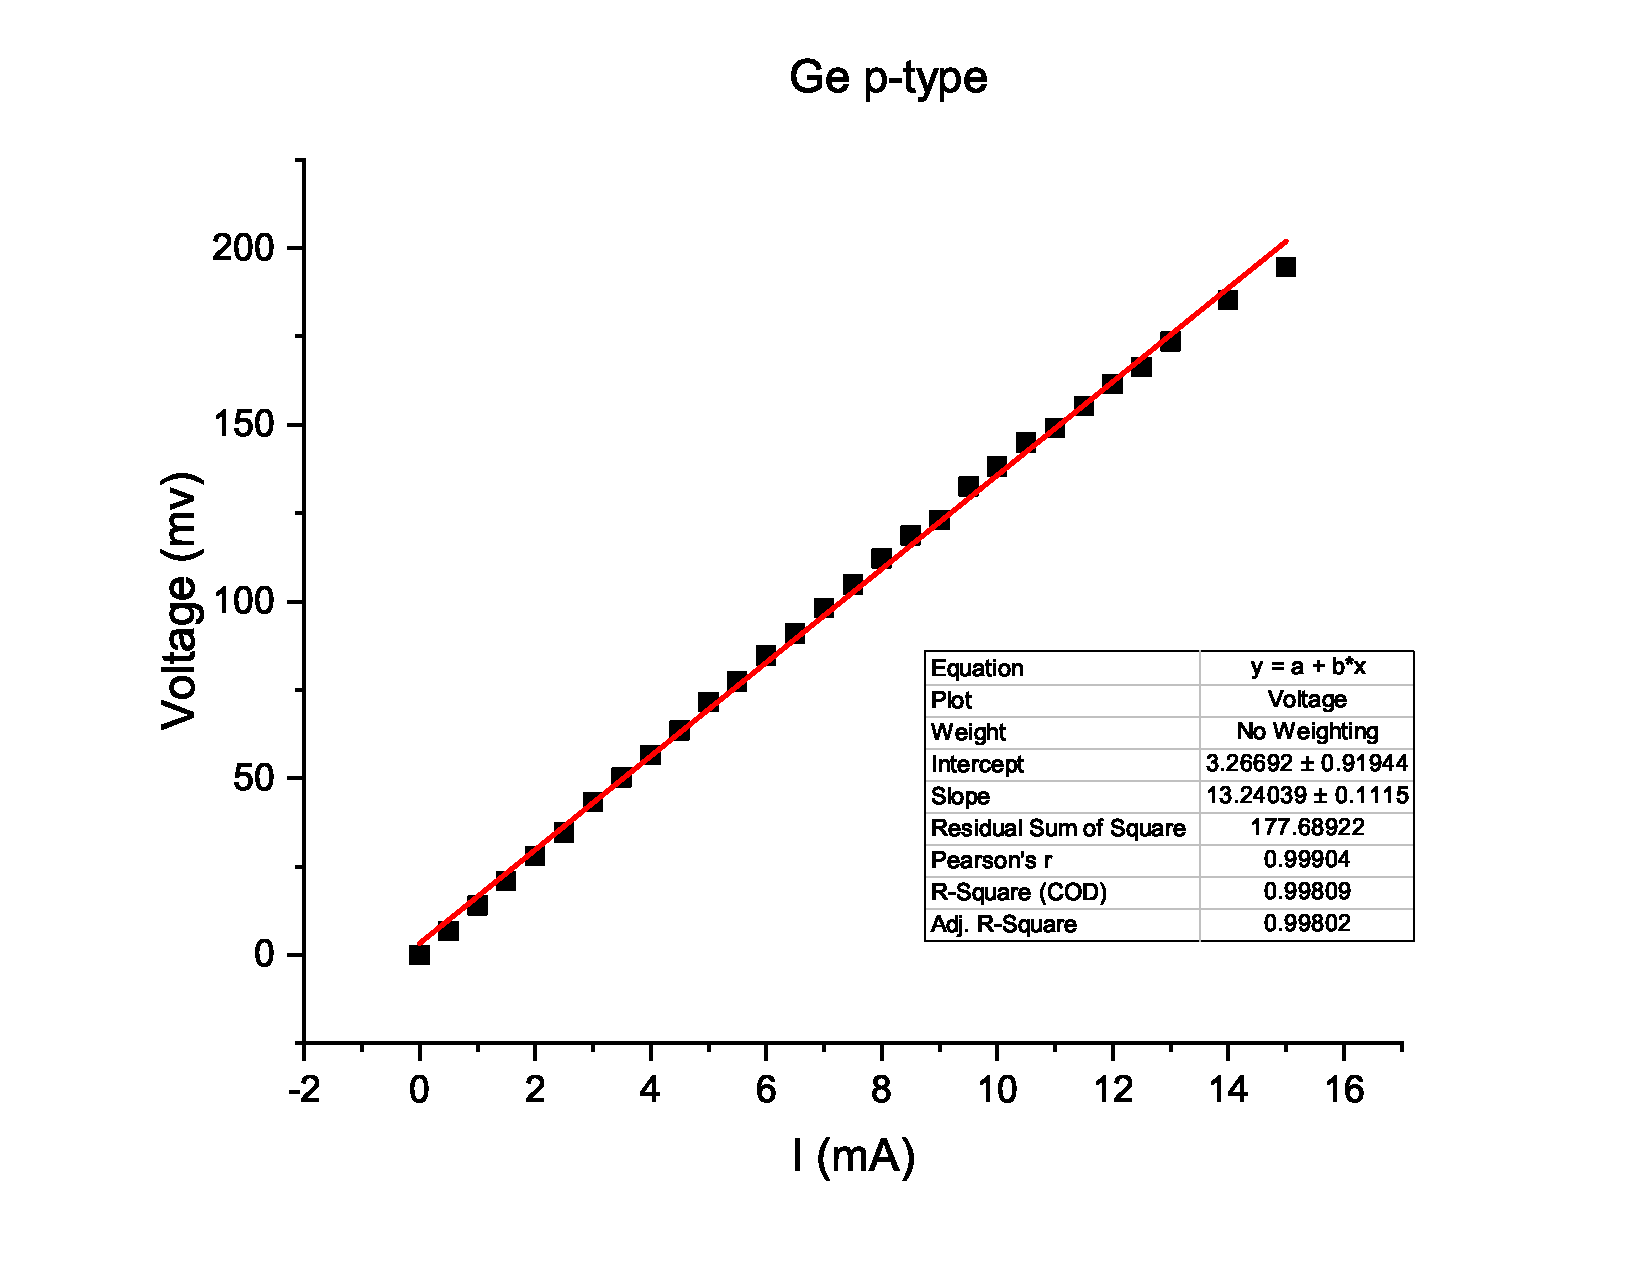
\includegraphics[width=0.9\columnwidth]{images/gep.eps}
				\caption{Hall voltage vs probe current for Ge p-type}
				\label{graph:3}
			\end{figure}

			We measured the Hall voltage at different probe current. The data is shown in Table \ref{tab:3}. The graph of Hall voltage vs probe current is shown in Fig \ref{graph:3}.

			from Graph \ref{graph:3}, we have $slope=\sfrac{V_y}{I_x}=-13.24$. Thus, using Equation \ref{eq:1} $ R_H=2.02 cm^3 coulomb^{-1}$
	\subsection{Temperature dependence of hall coefficient}
		\begin{itemize}
			\item sample thickness = $t=0.5mm$
			\item coil current = $I=3.07A$
			\item $H=2910G$
			\item probe current = $4.0 mA$
			\item Room temperature = $300K$
		\end{itemize}

		We measured the Hall voltage at different temperature. The data is shown in Table \ref{tab:4} and \ref{tab:5}. The graph of Hall coefficient vs temperature is shown in Fig \ref{graph}.

		\begin{figure}[h]
			\centering
			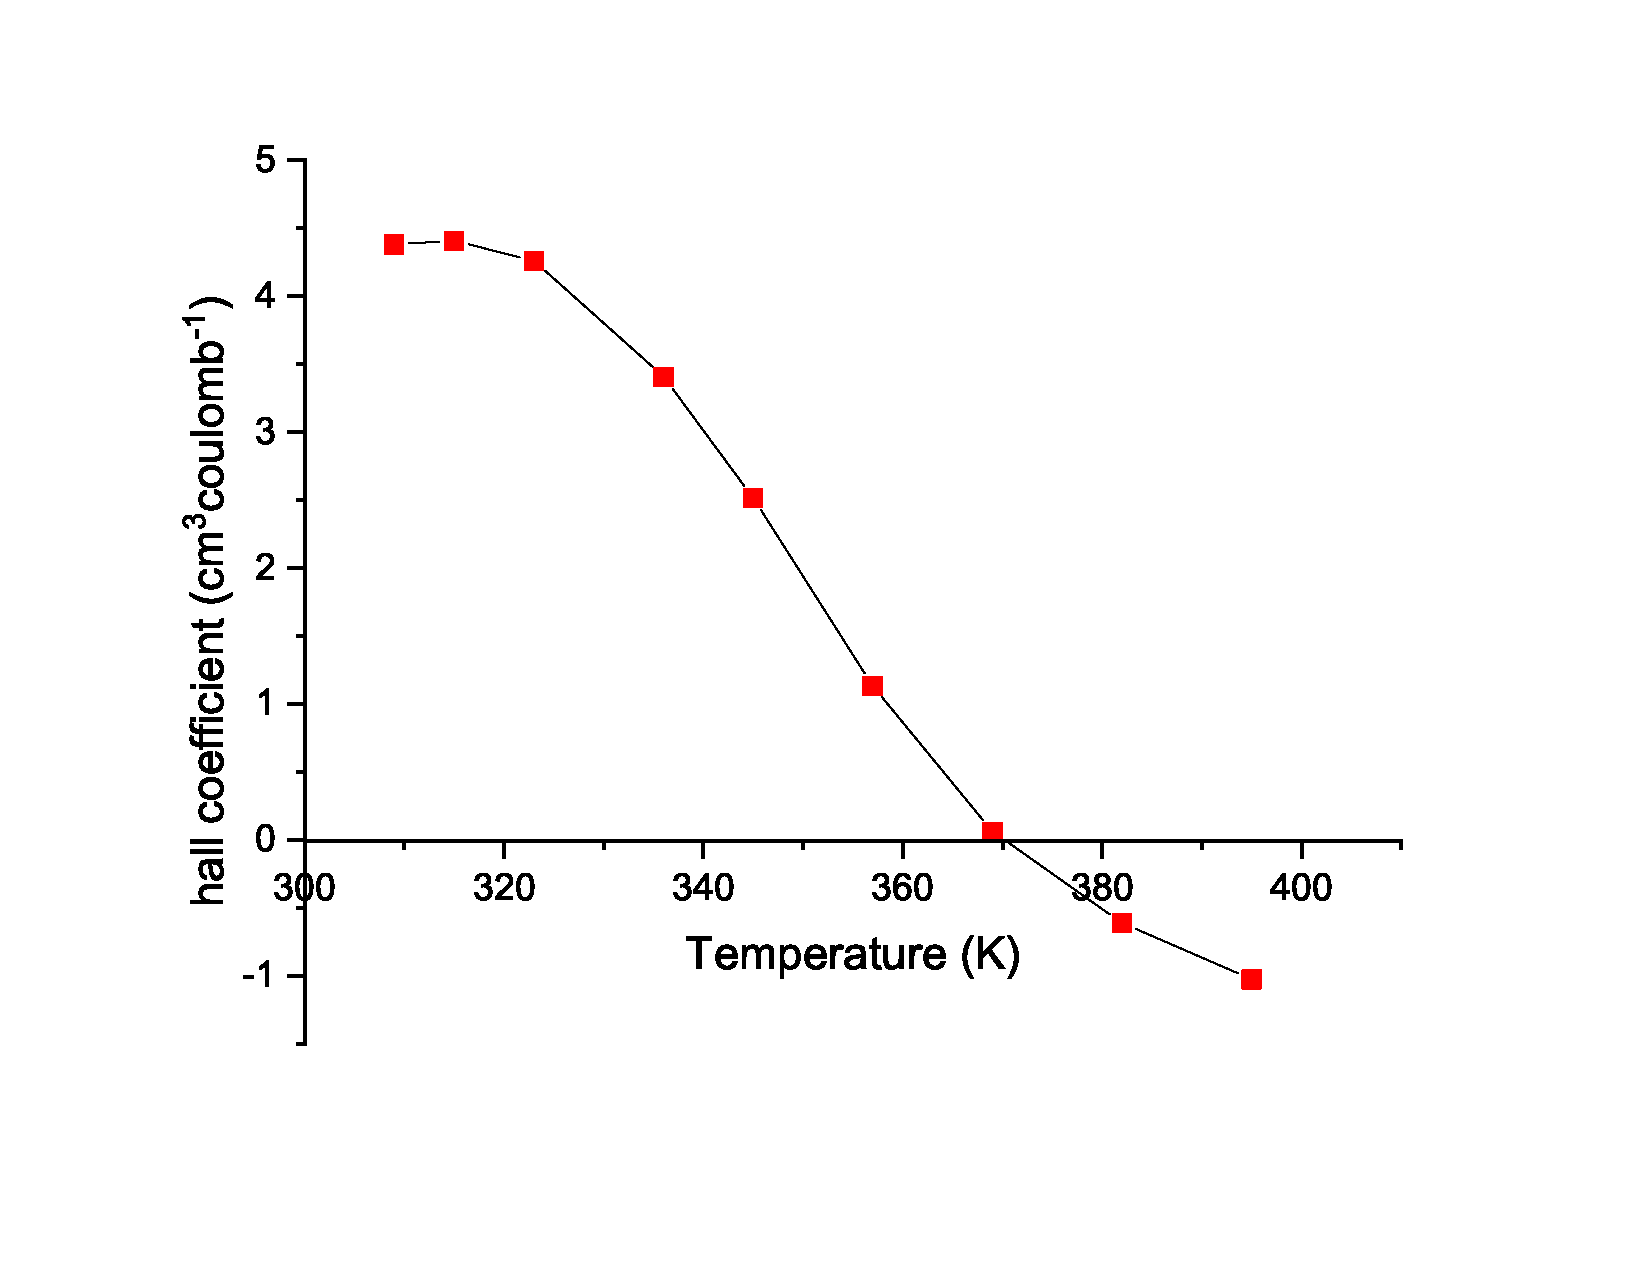
\includegraphics[width=0.9\columnwidth]{images/rh.eps}
			\caption{Hall coefficient vs. Temperature for Ge n-type}
			\label{graph}
		\end{figure}
		% Please add the following required packages to your document preamble:
% \usepackage{graphicx}
\begin{table}[]
	\centering
	\resizebox{\columnwidth}{!}{%
	\begin{tabular}{|c|c|c|c|c|}
	\hline
	\textbf{\begin{tabular}[c]{@{}c@{}}Heater\\ Current\end{tabular}} & \textbf{\begin{tabular}[c]{@{}c@{}}Thermal\\ EMF (mV)\end{tabular}} & \textbf{\begin{tabular}[c]{@{}c@{}}Hall\\ voltage (mV)\end{tabular}} & \textbf{\begin{tabular}[c]{@{}c@{}}Offset\\ voltage (mV)\end{tabular}} & \textbf{\begin{tabular}[c]{@{}c@{}}Voltage\\ (mV)\end{tabular}} \\ \hline
	304 & 0.35 & 145.4 & 43.4 & 102 \\ \hline
	405 & 0.6 & 146 & 43.4 & 102.6 \\ \hline
	501 & 0.91 & 142.6 & 43.4 & 99.2 \\ \hline
	605 & 1.43 & 122.7 & 43.4 & 79.3 \\ \hline
	706 & 1.8 & 102 & 43.4 & 58.6 \\ \hline
	802 & 2.32 & 69.8 & 43.4 & 26.4 \\ \hline
	900 & 2.81 & 44.8 & 43.4 & 1.4 \\ \hline
	1000 & 3.33 & 29.2 & 43.4 & -14.2 \\ \hline
	1100 & 3.9 & 19.5 & 43.4 & -23.9 \\ \hline
	\end{tabular}%
	}
	\caption{Hall voltage at different temperature}
	\label{tab:4}
\end{table}
		% Please add the following required packages to your document preamble:
% \usepackage{graphicx}
\begin{table}[h]
    \centering
    \resizebox{0.5\columnwidth}{!}{%
    \begin{tabular}{|c|c|}
    \hline
    \textbf{Temperature} & \textbf{Rh} \\ \hline
    309 & 4.3814433 \\ \hline
    315 & 4.40721649 \\ \hline
    323 & 4.26116838 \\ \hline
    336 & 3.40635739 \\ \hline
    345 & 2.51718213 \\ \hline
    357 & 1.13402062 \\ \hline
    369 & 0.06013746 \\ \hline
    382 & -0.60996564 \\ \hline
    395 & -1.0266323 \\ \hline
    \end{tabular}%
    }
    \caption{hall coefficient temperature dependance}
    \label{tab:5}
\end{table}